% !TeX root = main.tex

\hypertarget{introduction-to-functions}{%
\section{Introduction to Functions}\label{introduction-to-functions}}

\hypertarget{definition-and-notations}{%
\subsection{Definition and Notations}\label{definition-and-notations}}

A \textbf{\emph{relation}} is a set of ordered pairs. The set of all
first components of the ordered pairs is called the
\textbf{\emph{domain}}. The set of all second components of the ordered
pairs is called the \textbf{\emph{range}}.

A \textbf{\emph{function}} is a relation such that each element in the
domain corresponds to \textbf{exactly one} element in the range.

For a function, we usually use the variable \(x\) to represent an
element from the domain and call it the \textbf{\emph{independent
variable}}. The variable \(y\) is used to represent the value
corresponding to \(x\) and is called the \textbf{\emph{dependent
variable}}. We say \(y\) is a function of \(x\). When we consider
several functions together, to distinguish them we named functions by a
letter such as \(f\), \(g\), or \(F\). The notation \(f(x)\), read as
\textbf{``\(f\) of \(x\)'' or ``\(f\) at \(x\)''}, represents the output
of the function \(f\) when the input is \(x\).

The \textbf{\emph{domain}} of a function is the set of all allowed inputs. The \textbf{\emph{range}} of
a function is the set of all outputs.

\begin{example}

Find the indicated function value.

\begin{enumerate}[itemsep = 3.5\baselineskip]
\item
  \(f(-2)\),\quad \(f(x)=2x+1\)
\item
  \(g(2)\),\quad \(g(x)=3x^2-10\)
\item
  \(h(a-t)\),\quad \(h(x)=3x+5\).
\end{enumerate}

\end{example}


\hypertarget{graphs-of-functions}{%
\subsection{Graphs of Functions}\label{graphs-of-functions}}

\textbf{\emph{The graph of a function}} is the graph of its ordered
pairs. A graph of ordered pairs \((x,y)\) in the rectangular coordinate
system defines \(y\) as a function of \(x\) if any vertical line crosses
the graph at most once. This test is called the \textbf{\emph{vertical
line test}}.

\begin{example}

Determine which of the following graphs defines a function.\\
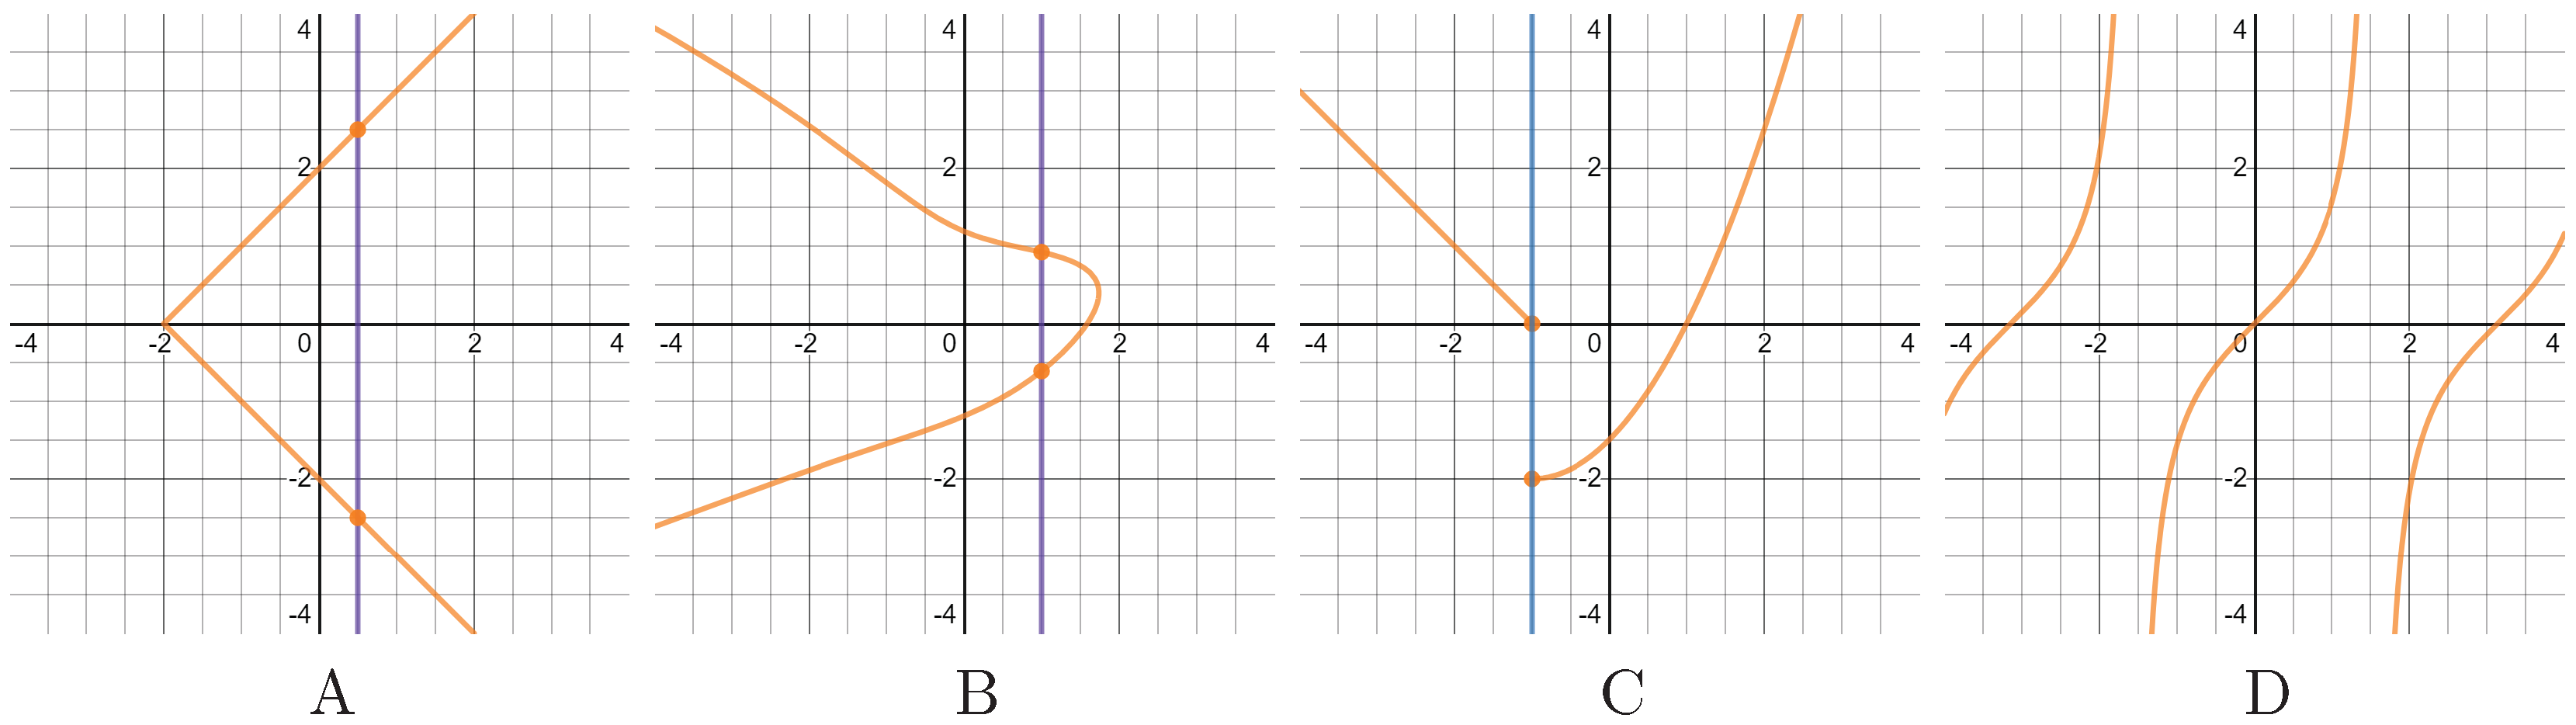
\includegraphics[width=\textwidth]{figs/four-graphs.png}
\end{example}
\vspace*{\baselineskip}

% 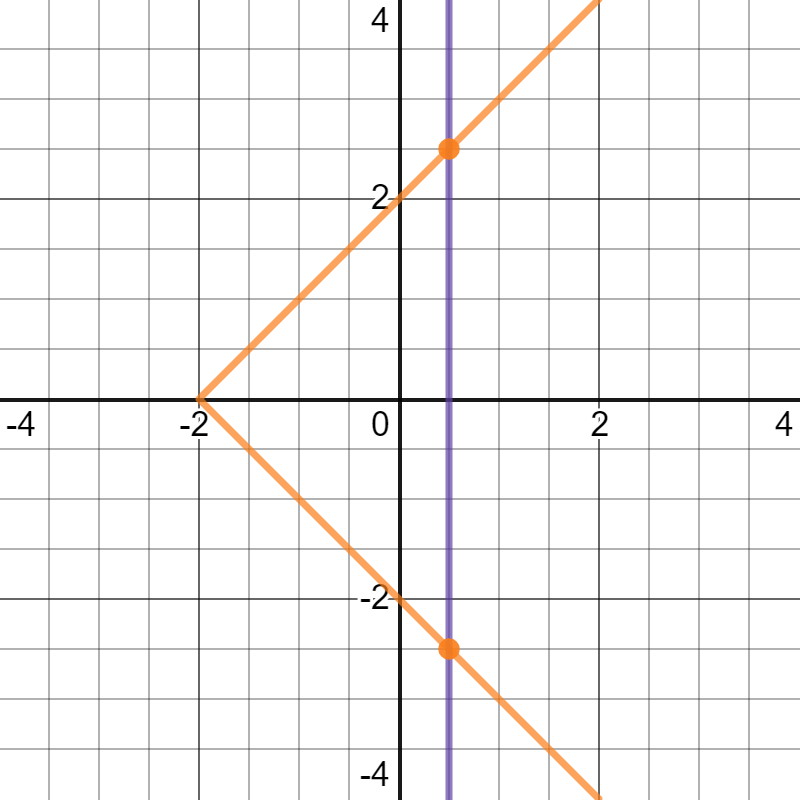
\includegraphics{figs/Graph-rotated-V.png}
% 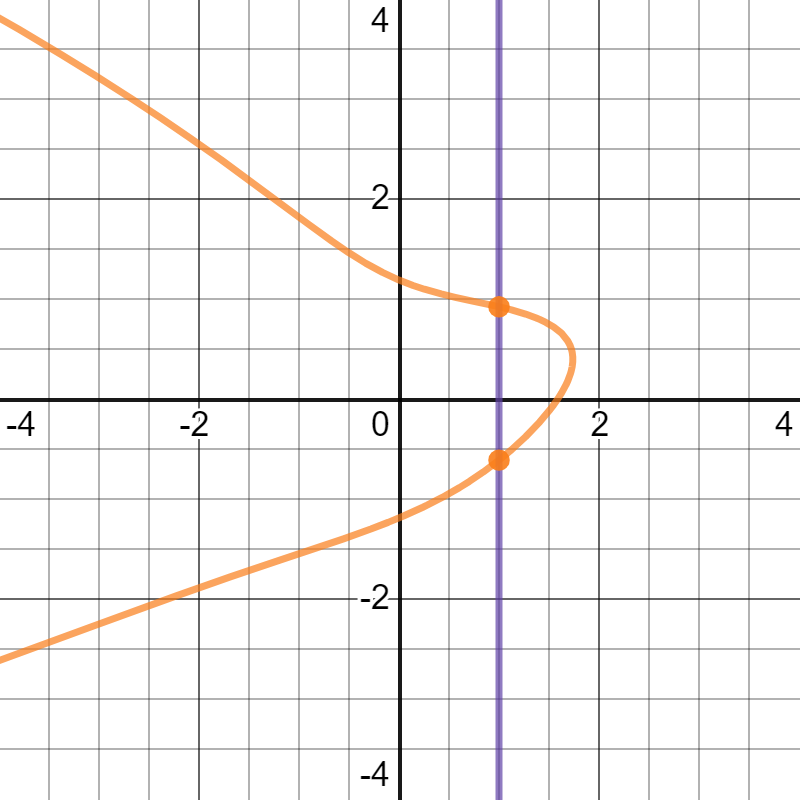
\includegraphics{figs/Graph-not-function-deg4.png}
% 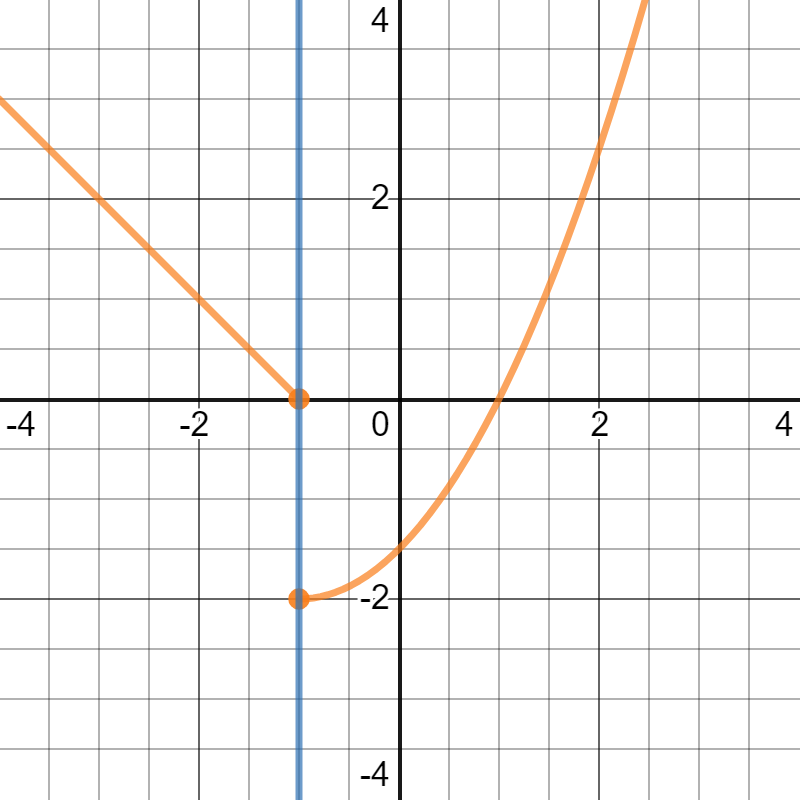
\includegraphics{figs/Graph-not-function-piecewise.png}
% 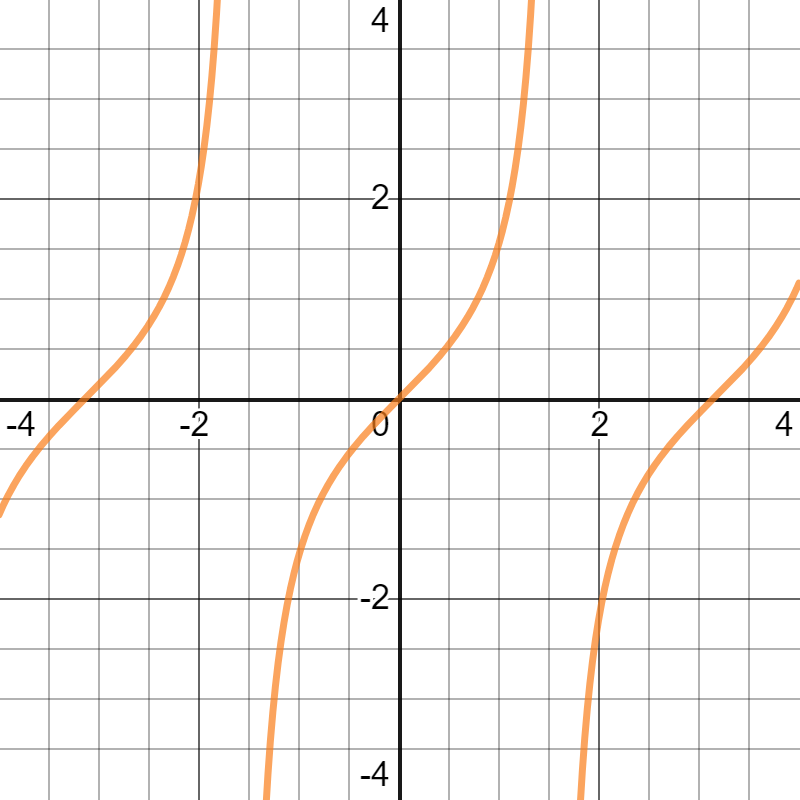
\includegraphics{figs/Graph-tanx.png}

\hypertarget{graph-reading}{%
\subsection{Graph Reading}\label{graph-reading}}


\begin{example}

Use the graph in the picture to answer the following questions.\\
\begin{fullwidth}
  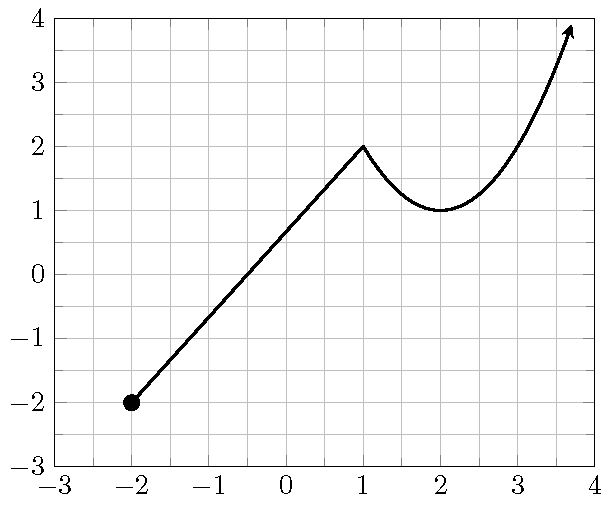
\includegraphics[width=0.8\linewidth]{figs/function-example-quadratic.png}
\end{fullwidth}

\begin{enumerate}[itemsep=2\baselineskip]
\item
  Determine whether the graph is a function and explain your answer.
\item
  Find the domain (in interval notation) of the graph.
\item
  Find the range (in interval notation) of the graph.
\item
  Find the interval where the graph is above \(2\).

\item
  Find the interval where the graph is is decreasing.

\item
  Find all maximum and minimum values of the function if they exist.
\item
  Find the value of \(y\) such that the point \((3, y)\) is on the
  graph.
\item
  Find the value of \(x\) such that \((x, 0)\) is on the graph.
\end{enumerate}

\end{example}



\subsection{Practice}

\begin{exercise}

Find the indicated function values for the functions \(f(x)=-x^2+x-1\)
and \(g(x)=2x-1\). Simplify your answer.

\begin{enumerate}[twocol]
\item
  \(f(2)\)
\item
  \(f(-x)\)
\item
  \(g(-1)\)
\item
  \(g(f(1))\)
\end{enumerate}
\end{exercise}

\begin{exercise}

Suppose \(g(x) = -3x + 1\).

\begin{enumerate}
\item
  Compute \(\dfrac{g(4)-g(1)}{4-1}\)
\item
  Compute \(\dfrac{g(x+h)-g(x)}{h}\)
\end{enumerate}

\end{exercise}

\begin{exercise}
Suppose the domain of the linear function \(l(x)=1-2x\) is \((0, 1)\).
Find the range of the function.
\end{exercise}
\vspace*{5\baselineskip}

\begin{exercise}

Use the graph in the picture to answer the following questions.
\\
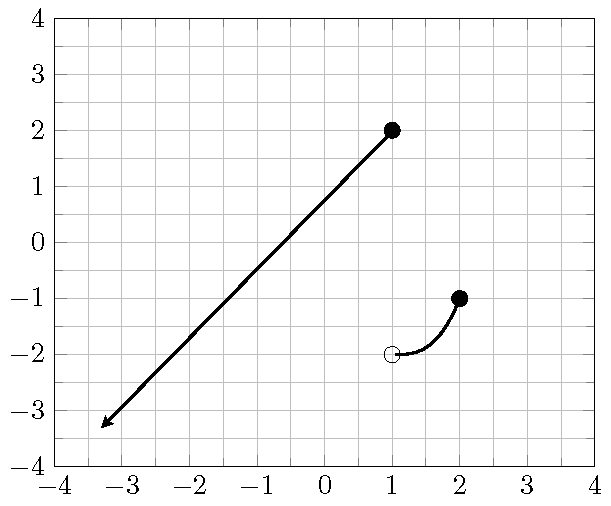
\includegraphics[width=0.8\textwidth]{figs/function-exercise-ray-cubic.png}

\begin{enumerate}[twocol]
\item
  Determine whether the graph is a function and explain your answer.
\item
  Find the domain of the graph (write the domain in interval notation).
\item
  Find the range of the graph (write the range in interval notation).

  \columnbreak

\item
  Find the interval where the graph is above the \(x\)-axis.
\item
  Find all points where the graph reaches a maximum or a minimum.
\item
  Find the values of the \(x\)-coordinate of all points on the graph
  whose \(y\)-coordinate is \(1\).
\end{enumerate}
\end{exercise}
\vspace*{2\baselineskip}

\begin{exercise}

Use the graph of the function \(f\) in the picture to answer the
following questions.
\\
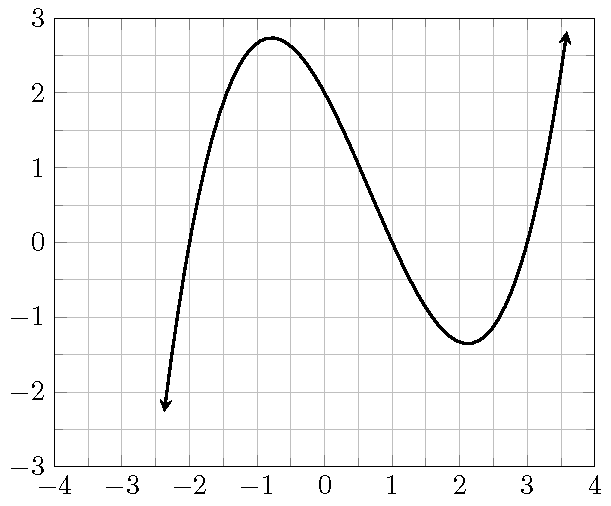
\includegraphics[width=0.8\textwidth]{figs/function-exercise-cubic.png}

\begin{enumerate}[twocol]
\item
  Find the \(y\)-intercept.
\item
  Find the value \(\dfrac{f(3)-f(0)}{3}.\)
\item
  Find the values \(x\) such that \(f(x)=0\).
\item
  Find the solution to the inequality \(f(x)>0\). Write in interval
  notation.
\end{enumerate}
\end{exercise}
\vspace*{2\baselineskip}

\begin{exercise}

Today Matt drove from home to school in 30 minutes. He spent 6 minutes
on local streets before driving on the highway and 4 minutes on local
streets towards school after getting off the highway. On local streets,
his average speed is 30 miles per hour. On the highway, his average
speed is 60 miles per hours.

\begin{enumerate}
\item
  Write the distance \(d\) (in miles) he drove as a function of the time
  \(t\) (in minutes)?
\item
  After 15 minutes, where was he and how far did he drive?
\item
  How far did he drive from home to school?
\end{enumerate}

\end{exercise}
